\documentclass[Serif, 10pt, brown]{beamer}
\usepackage{booktabs,xcolor}
\usepackage{pifont}
\newcommand*\CHECK{\ding{51}}
\usepackage{array}
\newcolumntype{P}[1]{>{\centering\arraybackslash}p{#1}}

\usepackage{setspace,mathtools,amssymb,multirow,array,amsmath,tikz}
\usepackage[normalsize]{subfigure}
\usetikzlibrary{patterns,automata,positioning,decorations.pathreplacing,decorations,calc}
\usepackage{curves}
\usepackage{caption}
\usepackage{wasysym}
\usepackage{epsfig,epstopdf,graphicx}

\curvewarnfalse

\newtheorem{proposition}{Proposition}
\theoremstyle{example}
\newtheorem{theoremh}{Theorem}
\theoremstyle{plain}
\renewcommand{\textfraction}{0.01}
\renewcommand{\floatpagefraction}{0.99}
\newcommand{\ul}{\underline}
\newcounter{units}
\setbeamercovered{dynamic}
\logo{\includegraphics[width=0.5in,keepaspectratio]{\FIGDIR/iitb_logo.png}}
\newcommand{\FIGDIR}{../figures} 
\newcommand{\RESULTDIR}{../../results} 
\mode<presentation>{
    \usetheme[right,currentsection,hideothersubsections]{UTD}
    \useoutertheme{sidebar}
    \useinnertheme[shadow]{rounded}
    \usecolortheme{whale}
    \usecolortheme{orchid}
    \usefonttheme[onlymath]{serif}
    \setbeamertemplate{footline}{\centerline{Slide \insertframenumber/\inserttotalframenumber}}
}

\usebeamercolor[fg]{author in sidebar}
\title[{Systems for LLMs}]{\sc Benchmarking and Performance Analysis of LLM Inferencing Systems}
\author[\ul{Saksham Rathi}]{{\textbf{Saksham Rathi}}}
\institute[UTD]{\sc\small Systems for LLMs\\ Under Prof. Mythili Vutukuru}
\date[UCI]{Indian Institute of Technology Bombay \\ Autumn 2025-26}

\begin{document}
\frame{\titlepage}

\begin{frame}{Contents}
	\tableofcontents
\end{frame}

\section{Various Scheduler Designs}
\subsection{vLLM Schedulers}
\begin{frame}{First Come First Serve Policy}
    \begin{itemize}
        \item Adds requests one by one, from the core engine into a waiting queue
        \item The requests are extracted in a first come first serve manner
        \item We stop selecting requests from the waiting queue into the running batch, once the size reaches \texttt{max\_batch\_size}
    \end{itemize}
\end{frame}

\begin{frame}{Priority Based}
    \begin{itemize}
        \item The user passes priority values along with the requests' strings themselves
        \item We use a min heap to find the request with the smallest priority value (executed at first)
        \item Ties are broken in a first come first serve manner (through tracking request's arrival time)
    \end{itemize}
\end{frame}

\subsection{Our Schedulers}
\begin{frame}{Greedy First Come First Serve}
    \begin{itemize}
        \item We keep a track of the working set along with the requests we add to the current running scheduler batch
        \item We add requests in a first come first serve manner
        \item However, now we are also controlling the batch size - we stop whenever addition of the next request increases the working set size beyond a threshold (decided by L2 cache size)
        \item For our workload, and GPU - it boils down to stopping whenever the next request belongs to a different family
    \end{itemize}
\end{frame}

\begin{frame}{Greedy First Come First Serve - Appendix - Expected Batch Size}
    Let's say we have $N$ families. The user passes a bunch of requests, which can belong to any of these families. Moreover, all the requests have been shuffled, such that the probability of a request at position $i$ to be of family $j$ is exactly $\frac{1}{N}$.

    Assume that the first request belongs to family $j$. We find out the expected value of the size of the first scheduler batch.

    For the batch to have size exactly $x$:
    \begin{itemize}
        \item The first $x - 1$ requests after the initial one must also be of family $j$.
        \item The $x$-th request must be of a different family.
    \end{itemize}


    The probability that the batch is of size $x$ is given by:
    \[
        \Pr[X = x]
        = \left(\frac{1}{N}\right)^{x-1} \cdot \frac{N-1}{N}, \quad x \ge 1.
    \]
\end{frame}



\begin{frame}{Greedy First Come First Serve - Appendix - Expected Batch Size}
    Let $X$ denote the size of the first batch. Its expected value is:
    \[
        \mathbb{E}[X]
        = \sum_{x=1}^{\infty} x \Pr[X = x]
        = \sum_{x=1}^{\infty} x \left(\frac{1}{N}\right)^{x-1} \frac{N-1}{N}.
    \]
    Using the identity
    \[
        \sum_{x=1}^{\infty} x r^{x-1} = \frac{1}{(1-r)^2}, \quad |r| < 1,
    \]
    with $r = \frac{1}{N}$, we obtain:
    \[
        \mathbb{E}[X]
        = \frac{N-1}{N} \cdot \frac{1}{\left(1 - \frac{1}{N}\right)^2}
        = \frac{N}{N-1}.
    \]

    \vspace{0.3cm}
    \[
        \boxed{\mathbb{E}[\text{batch size}] = \frac{N}{N-1}}
    \]

    For example, when we have 2 families, the expected batch size would be just 2.
\end{frame}


\begin{frame}{Family ID Based}
    \begin{itemize}
        \item If we can set priority values for each of the request, then why can't we set the family to which they belong to?
        \item We have separate queues for each family
        \item All the individual queues operate in a first come first serve manner
        \item If there is a request of family ID $j$ already present in the scheduler batch, then we try to add all the requests of that family in the same batch (till we hit \texttt{max\_batch\_size}). If there is no request of that family available, then we stick to the current batch (no more requests added)
        \item So, the batch size is no longer static - it is dynamically set in accordance with the workload
    \end{itemize}
\end{frame}

\begin{frame}{Radix Tree Based}
    \begin{itemize}
        \item Key idea: Instead of treating each request independently, we exploit shared token prefixes across requests
        \item Each request is represented as a path of tokens in a radix tree
        \item Internal nodes correspond to shared token substrings 
        \item The scheduler maintains a working set of active nodes (tokens already materialized / cached)
        \item Each waiting request has a cost = number of tokens missing from the working set
    \end{itemize}
\end{frame}

\begin{frame}{Radix Tree Based}
    To schedule the next request:
    \begin{itemize}
        \item We start from leaves already in the working set
        \item Traverse upwards toward the root
        \item At each node, we look for waiting requests passing through it
        \item We select the request with minimum missing-token cost
    \end{itemize}
    Activating a request:
    \begin{itemize}
        \item Adds its path to the working set
        \item Future requests that share prefixes become cheaper
        \item This dynamically forms prefix-coherent batches, minimizing recomputation
    \end{itemize}
\end{frame}


\begin{frame}{Radix Tree Based - Radix Tree Construction}
\centering
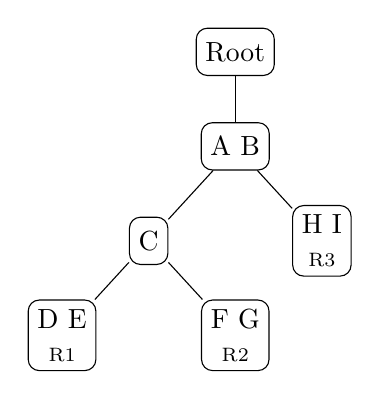
\begin{tikzpicture}[
    every node/.style={draw, rectangle, rounded corners, minimum height=6mm, align=center},
    level distance=12mm,
    sibling distance=22mm
]

\node {Root}
    child {
        node {A B}
        child {
            node {C}
            child {
                node {D E\\{\scriptsize R1}}
            }
            child {
                node {F G\\{\scriptsize R2}}
            }
        }
        child {
            node {H I\\{\scriptsize R3}}
        }
    };

\end{tikzpicture}

\vspace{1em}
\small
Each leaf corresponds to a request.  
Internal nodes represent shared token prefixes.
\end{frame}

\begin{frame}{Radix Tree Based - Working Set After Activation}
\centering
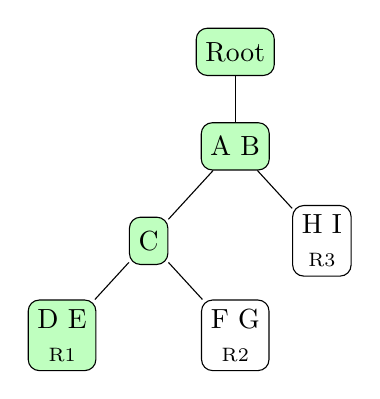
\begin{tikzpicture}[
    every node/.style={draw, rectangle, rounded corners, minimum height=6mm, align=center},
    ws/.style={fill=green!25},
    level distance=12mm,
    sibling distance=22mm
]

\node[ws] {Root}
    child {
        node[ws] {A B}
        child {
            node[ws] {C}
            child {
                node[ws] {D E\\{\scriptsize R1}}
            }
            child {
                node {F G\\{\scriptsize R2}}
            }
        }
        child {
            node {H I\\{\scriptsize R3}}
        }
    };

\end{tikzpicture}

\vspace{1em}
\small
Green nodes indicate the working set after activating R1.
\end{frame}

\begin{frame}{Radix Tree Based - Finding the Best Request}
\centering
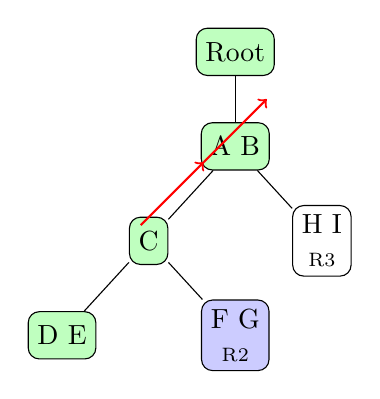
\begin{tikzpicture}[
    every node/.style={draw, rectangle, rounded corners, minimum height=6mm, align=center},
    ws/.style={fill=green!25},
    candidate/.style={fill=blue!20},
    level distance=12mm,
    sibling distance=22mm
]

\node[ws] {Root}
    child {
        node[ws] {A B}
        child {
            node[ws] {C}
            child {
                node[ws] {D E}
            }
            child {
                node[candidate] {F G\\{\scriptsize R2}}
            }
        }
        child {
            node {H I\\{\scriptsize R3}}
        }
    };

\draw[->, thick, red] (-1.2,-2.2) -- (-0.4,-1.4);
\draw[->, thick, red] (-0.4,-1.4) -- (0.4,-0.6);

\end{tikzpicture}

\vspace{1em}
\small
Traversal starts from working-set leaves and moves upward.  
R2 is selected due to maximum prefix overlap.
\end{frame}


\begin{frame}{Radix Tree Based - Dynamic Batch Growth}
\centering
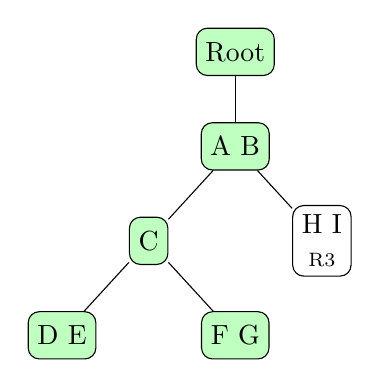
\begin{tikzpicture}[
    every node/.style={draw, rectangle, rounded corners, minimum height=6mm, align=center},
    ws/.style={fill=green!25},
    level distance=12mm,
    sibling distance=22mm
]

\node[ws] {Root}
    child {
        node[ws] {A B}
        child {
            node[ws] {C}
            child {
                node[ws] {D E}
            }
            child {
                node[ws] {F G}
            }
        }
        child {
            node {H I\\{\scriptsize R3}}
        }
    };

\end{tikzpicture}

\vspace{1em}
\small
Batch size grows dynamically as long as marginal cost is low.
\end{frame}

\begin{frame}{Radix Tree Based - Issues}
    The above approach has a few issues:
    \begin{itemize}
        \item Adding a request is quite costly - there might be splitting/merging of nodes. Although finding the best request is quite efficient
        \item Each request may contain thousands of tokens, so the tree depth might get quite large too
        \item We cannot have a parallel thread/process handling the radix tree, because maintaining sync is difficult. What if we removed a request, from our waiting queue, but it takes some time to remove it from the radix tree?
    \end{itemize}
\end{frame}

\begin{frame}{Chunked Hash Tree Based}
\begin{itemize}
    \item Requests are represented using \textbf{hashed cumulative prefixes}
    \item Tokens are divided into fixed-size chunks
    \item Each level corresponds to \texttt{hash(tokens[0:k])}
    \item No explicit tree structure or node splitting
    \item Much faster than radix trees for large workloads
\end{itemize}
\end{frame}

\begin{frame}{Chunked Hash Tree Based - Working Set}
\begin{itemize}
    \item Working set = set of active \textbf{(level, hash)} pairs
    \item Each active request contributes all its prefix hashes
    \item Request cost = number of missing prefix hashes
    \item Scheduling prefers requests with minimal missing chunks
    \item Enables dynamic batch growth similar to radix trees
\end{itemize}
\end{frame}


\begin{frame}{Chunked Hash Tree Based - Insertion}
\centering
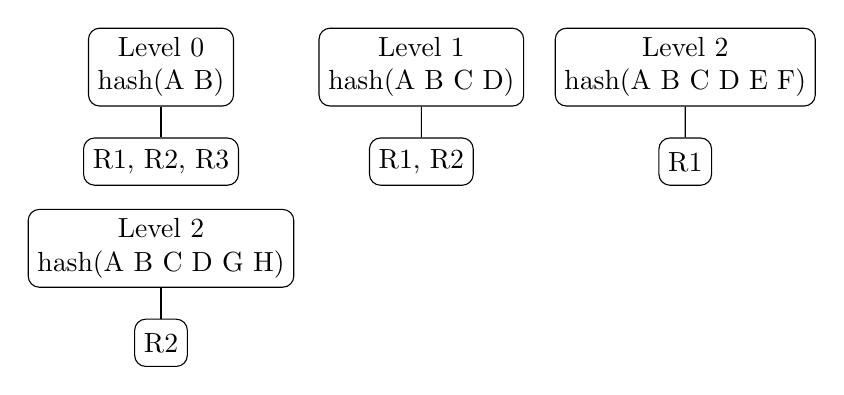
\begin{tikzpicture}[
    every node/.style={draw, rectangle, rounded corners, minimum height=6mm, align=center},
    level distance=12mm,
    sibling distance=32mm
]

\node {Level 0\\hash(A B)}
    child { node {R1, R2, R3} };

\node[right=2cm] {Level 1\\hash(A B C D)}
    child { node {R1, R2} };

\node[right=5cm] {Level 2\\hash(A B C D E F)}
    child { node {R1} };


\node[right=8cm, below=1.8cm] {Level 2\\hash(A B C D G H)}
    child { node {R2} };

\end{tikzpicture}

\vspace{0.5em}
\small
Each level stores hashes of cumulative token prefixes.
\end{frame}


\begin{frame}{Chunked Hash Tree Based - Working Set}
\centering
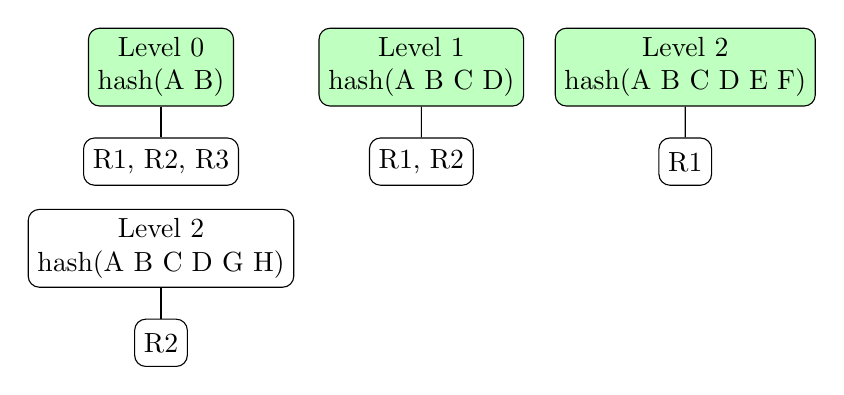
\begin{tikzpicture}[
    every node/.style={draw, rectangle, rounded corners, minimum height=6mm, align=center},
    ws/.style={fill=green!25},
    level distance=12mm,
    sibling distance=32mm
]

\node[ws] {Level 0\\hash(A B)}
    child { node {R1, R2, R3} };

\node[ws, right=2cm] {Level 1\\hash(A B C D)}
    child { node {R1, R2} };

\node[ws, right=5cm] {Level 2\\hash(A B C D E F)}
    child { node {R1} };

\node[right=8cm, below=1.8cm] {Level 2\\hash(A B C D G H)}
    child { node {R2} };

\end{tikzpicture}

\vspace{0.5em}
\small
Green boxes indicate prefix hashes in the working set.
\end{frame}


\begin{frame}{Chunked Hash Tree Based - Best Request Selection}
\centering
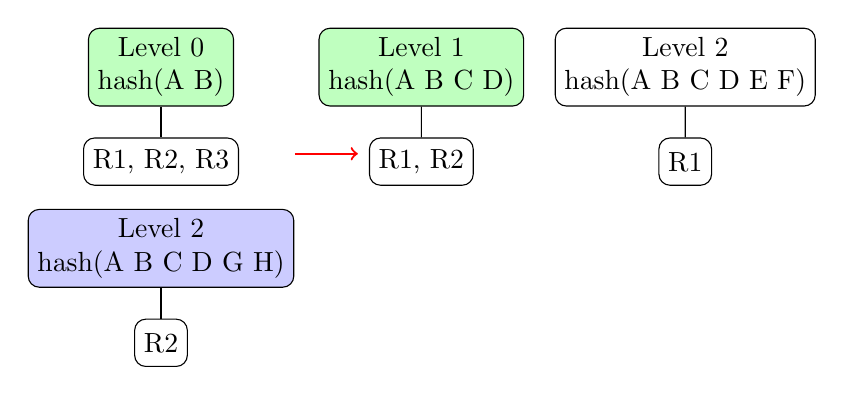
\begin{tikzpicture}[
    every node/.style={draw, rectangle, rounded corners, minimum height=6mm, align=center},
    ws/.style={fill=green!25},
    candidate/.style={fill=blue!20},
    level distance=12mm,
    sibling distance=32mm
]

\node[ws] {Level 0\\hash(A B)}
    child { node {R1, R2, R3} };

\node[ws, right=2cm] {Level 1\\hash(A B C D)}
    child { node {R1, R2} };

\node[right=5cm] {Level 2\\hash(A B C D E F)}
    child { node {R1} };

\node[candidate, right=8cm, below=1.8cm]
    {Level 2\\hash(A B C D G H)}
    child { node {R2} };

\draw[->, thick, red] (1.7,-1.1) -- (2.5,-1.1);

\end{tikzpicture}

\vspace{0.5em}
\small
R2 is selected since it has maximum prefix overlap with the working set.
\end{frame}

\subsection{Already Existing Schedulers}


\section{Throughput Numbers}


\section{}
\begin{frame}
    \Huge{\centerline{\bf Thank You}}
\end{frame}

\end{document}
